\chapter{Our Work}
\label{chap:prelim-exp}

\section{Overview}
This work presents a method dealing with challenges where we have a fully annotated dataset, however very small in size, and a large dataset but weakly annotated. We aim to overcome these challenges by implementing a hybrid approach for semantic segmentation of lymphocyte cells. Firstly we try to train and validate a model on the small dataset itself. Then we use preprocessing and computer vision techniques to generate various pseudo-mask sets out of bounding-box annotations for the weakly annotated dataset and train a model on it, which is again validated on the small, fully annotated dataset. Then we try to identify and select the best fusing strategy for the masks sets, in order to utilize different abilities of the sets to capture the cell region. Next we select the best model (with the most successful mask fusing strategy) and fine-tune it using a portion of data in the fully annotated dataset. We evaluate each of these experiments with Dice score and IoU, and also create a confusion matrix for the final model, displaying what cell types were most confusing it. We start with the fundamental part - the description of the datasets used.

\section{Datasets}
\label{sec:datasets}

\paragraph{TIGER} In our work, we use the TIGER dataset which was released with the challenge under the same name on the Grand Challenge platform \cite{tiger_dataset}. It contains H\&E stained WSIs of Her2 positive and TNBC breast cancer tissues obtained by core needle biopsies or surgical resections. The images were scanned using 20x magnification. The dataset is released in three formats. We work with the one called WSIROIS. The WSIs come from three different institutions:

\begin{enumerate}
    \item TCGA (151 WSIs) dataset, contains images of TNBC from the TCGA-BRCA archive, annotations and magnification were adopted to be in line with those used further.
    \item RUMC (26 WSIs) images of both TNBC and Her2 positive breast cancer obtained from Radboud University Medical Center in the Netherlands, annotated by a panel of board-certified pathologists.
    \item JB (18 WSIs) images of both TNBC and Her2 positive breast cancer obtained from Jules Bordet Institute in Belgium, annotated by a panel of board-certified pathologists.
\end{enumerate}

The RUMC and JB WSIs contain 3 annotated ROIs with a size of approximately $500\!\times\!500$ \textmu m. The WSIs obtained from TCGA are more specific. This dataset was created by merging two other datasets: the BCSS (151 WSIs) and the NuCLS (124 WSIs). The NuCLS is a subset of the BCSS dataset. In the BCSS dataset, the tissue in a single large ROI is annotated but no cells are annotated. In the NuCLS a variable number of smaller ROIs are selected within the large ROI (same large ROI as in the BCSS) and these are densely annotated for multiple cell types. Annotations are adapted to match the other used annotations, as was mentioned.

The WSIROIS format contains:

\begin{itemize}
    \item WSI level annotations, wherein each WSI contains manual annotations of ROIs. Different tissue types are annotated with polygons, namely: invasive tumor, tumor-associated stroma, in-situ tumor, healthy glands, necrosis not in-situ, inflamed stroma, and rest. Most ROIs have also annotated plasma cells and lymphocytes. These were annotated using point annotations and then a bounding box was constructed and centered on the point of annotation with the size of $6\!\times\!6$ \textmu m, $8\!\times\!8$ \textmu m, or $9\!\times\!9$ \textmu m. Annotations for WSIs are released in XML format and also as a multi-resolution TIF image.
    \item ROI level annotations, where authors cropped the ROIs from WSIs and stored them as PNG files. Tissue type annotations are released as PNG images, containing pixel-level masks, and cell annotations are released in the COCO format - a JSON file containing file paths (the PNG images of ROIs) with IDs and metadata and corresponding annotations of bounding box position and size.
\end{itemize}

We further work with the part of the dataset that has ROI-level annotations. This part of the dataset consists of 1,879 (1,744 from TCGA, 81 from RUMC, 54 from JB) ROIs cropped from 44 (124 from TCGA, 26 from RUMC, 18 from JB). Together they contain 30,524 annotated cell nuclei.

An example of an image and its bounding box labels can be seen in Figure \ref{fig:tiger-with-without}.

\begin{figure}[H]
  \centering
  \begin{subfigure}[b]{0.32\textwidth}
    \centering
    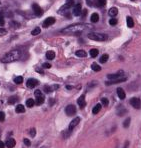
\includegraphics[width=\linewidth]{assets/images/for_presentation/image_TCGA-EW-A1P8-01Z-00-DX1.E9852193-8CDD-49EF-B49B-DA6931198F0D_[8391, 13690, 8532, 13838].png}
    \subcaption{Without annotations}\label{fig:tiger-img}
  \end{subfigure}%
  \quad
  \begin{subfigure}[b]{0.32\textwidth}
    \centering
    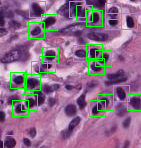
\includegraphics[width=\linewidth]{assets/images/for_presentation/bbox_TCGA-EW-A1P8-01Z-00-DX1.E9852193-8CDD-49EF-B49B-DA6931198F0D_[8391, 13690, 8532, 13838].png}
    \subcaption{With annotations}\label{fig:tiger-bbox}
  \end{subfigure}%
  \caption{Example of TIGER image without and with annotations of TILs \cite{tiger_dataset}}
  \label{fig:tiger-with-without}
\end{figure}

\paragraph{TNBC} Triple Negative Breast Cancer Nuclei Segmentation dataset \cite{TNBC-nuclei-seg}, is an open dataset consisting of 11 patients with breast cancer, with varying numbers of images for each patient, provided regions of interest (ROIs) PNGs. Together, it has 50 annotated ROIs of size 512x512, scanned with the 40x magnification. Specifically, we use the extended version of this dataset \cite{TNBC-nuclei-seg-extended}, where annotations of cell classes were added. Each image has a corresponding pixel mask, where each pixel is labeled by the class it represents. There are 11 different cell classes plus background and unknown class. We also note that this extended version of the dataset provides images of brain tissue, but since it is not part of our work, we only work with the images of breast cancer. An example image with its ground truth mask, already relabeled so only lymphocytes are annotated, can be seen in figure \ref{fig:tcga-with-without}.

\begin{figure}[H]
  \centering
  \begin{subfigure}[b]{0.32\textwidth}
    \centering
    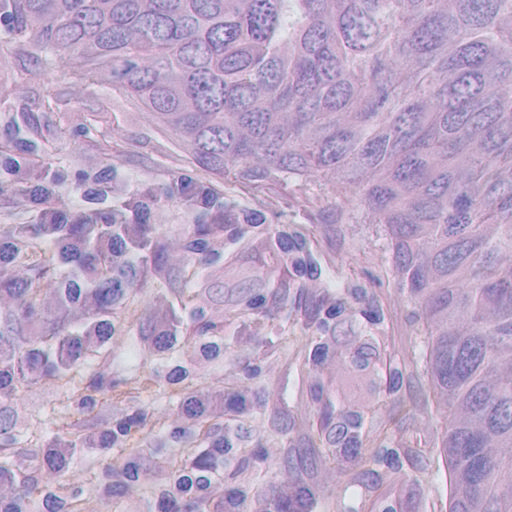
\includegraphics[width=\linewidth]{assets/images/for_presentation/image_10_1.png}
    \subcaption{Image}\label{fig:tcga-img}
  \end{subfigure}%
  \hfill
  \begin{subfigure}[b]{0.32\textwidth}
    \centering
    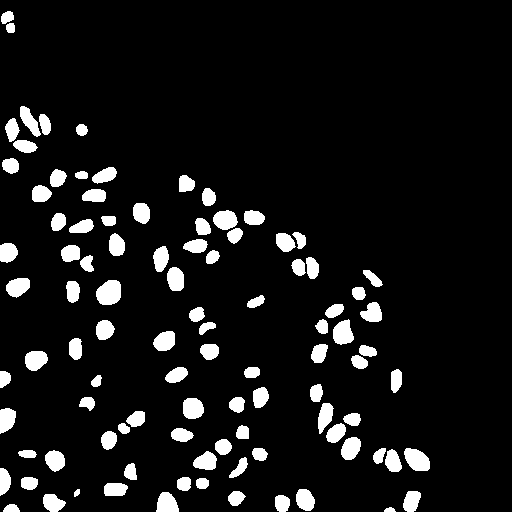
\includegraphics[width=\linewidth]{assets/images/for_presentation/mask_10_1.png}
    \subcaption{Mask}\label{fig:tcga-mask}
  \end{subfigure}%
  \hfill
  \begin{subfigure}[b]{0.32\textwidth}
    \centering
    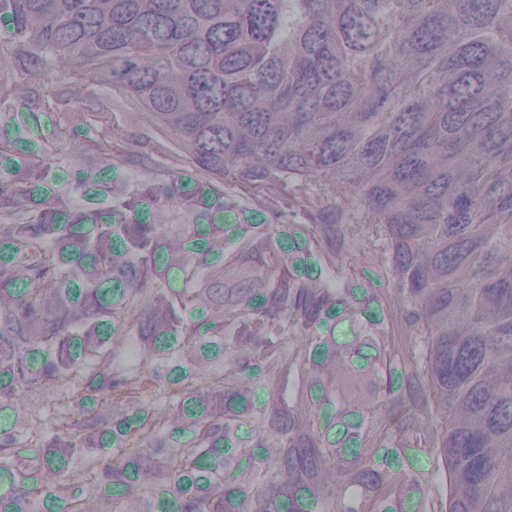
\includegraphics[width=\linewidth]{assets/images/for_presentation/overlay_10_1.png}
    \subcaption{Image with mask overlay}\label{fig:tcga-overlay}
  \end{subfigure}%
  \caption{Example of TNBC image, mask and overlay, where TILs are annotated \cite{TNBC-nuclei-seg-extended}}
  \label{fig:tcga-with-without}
\end{figure}

\section{Deep Learning Model Architecture}
As a deep learning model, we employ the U-Net architecture. U-Net is a powerful architecture, and as we mention in Chapter \ref{chapter:dnn} it is also widely used in the medical imaging domain. Specifically, we use the ResNet-34 encoder as the U-Net's backbone, which is already pretrained on the ImageNet dataset. This choice was based on the fact that residual blocks further improve the U-Net's ability to learn, as we write in Chapter \ref{chapter:dnn}. In the state-of-the-art, which we present in Chapter \ref{chapter:related}, authors in \cite{Zhang2022, Liang2023} also use ResNet architectures, and specifically, ResNet-34 is used in \cite{Lin2023}. The inspiration to initialize the encoder with weights pretrained on the ImageNet dataset came from the state-of-the-art works as well, where a similar approach was used in \cite{Zhang2022, Lin2023, Liang2023}. The full architecture of the model can be seen in Figure \ref{fig:our-architecture}.

\begin{figure}[H]
\begin{centering}
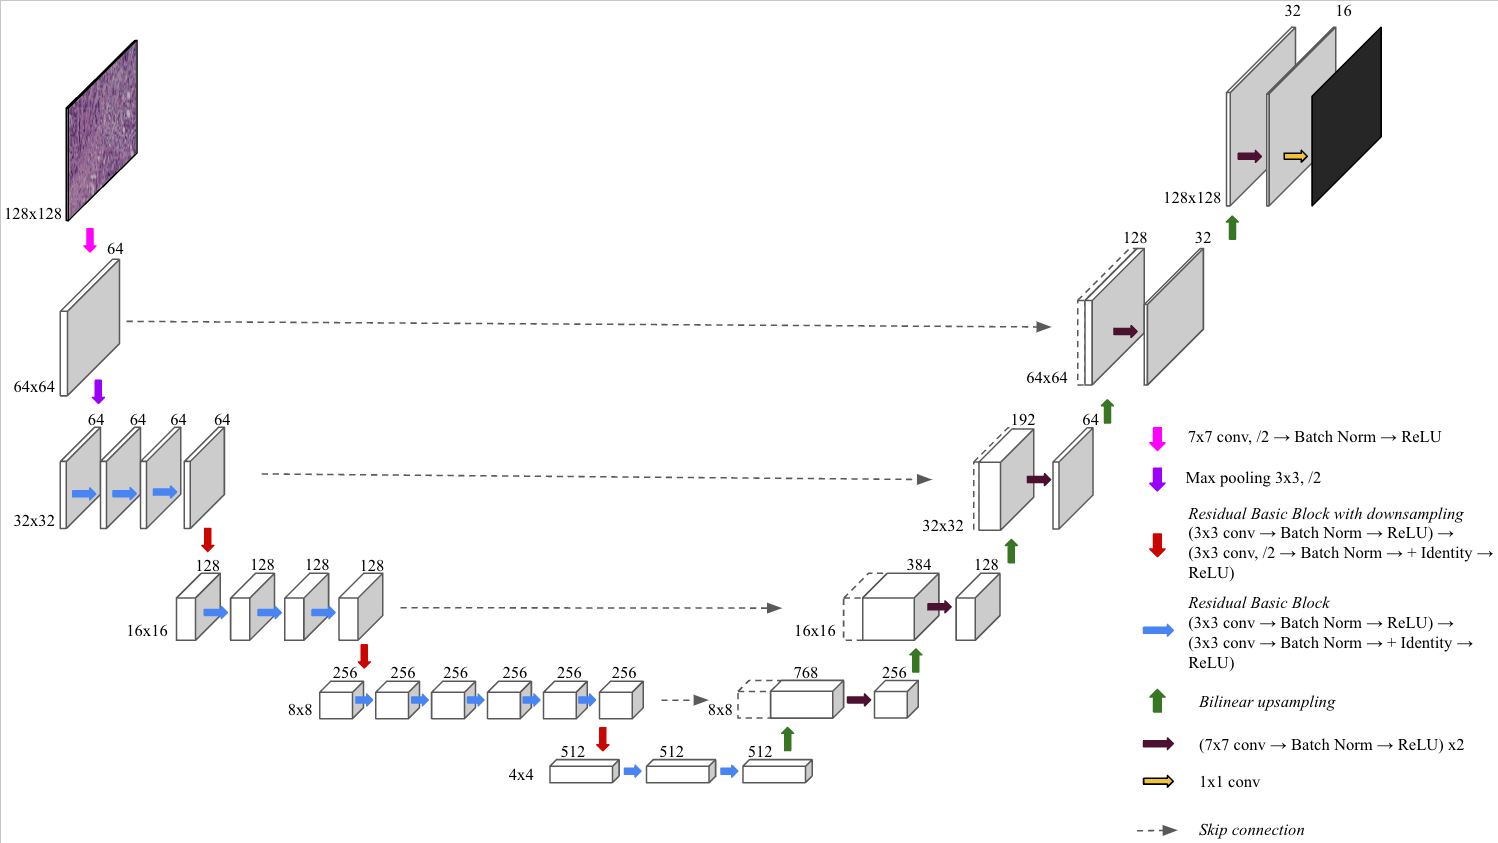
\includegraphics[width=\textwidth]{assets/images/for_presentation/our_architecture.png}
\par\end{centering}
\caption{The architecture of our model 
\label{fig:our-architecture}}
\end{figure}

This model is being used in all our experiments as the segmentation model. The training setup and model's hyperparameters remain the same in every experiment as well. The input for the model is an image of size $128\times128$ pixels in a 3 - RGB - channel space. The model's segmentation head produces a binary mask of size $128\times128$ pixels and depth of 1. The output mask is then run through the sigmoid function, to squeeze the values between 0 and 1. A threshold of 0.5 is applied to this mask as pixels with value less then 0.5 are predicted background and labeled with number 0 and pixels with value greater than or equal to 0.5 are predicted TILs and labeled with number 1.

\subsection{Training}


\section{Data Preprocessing}
Since we work with two very distinct datasets, and furthermore, the TIGER dataset is composed of three other datasets, we need to employ a robust preprocessing framework in order to align all datasets on the same level.

\subsection{Normalization} 
TIGER and TNBC datasets pose several challenges to us. Firstly, as we described in section \ref{sec:datasets}, data come from four distinct sources (three for TIGER and one for TNBC) - this means that the staining is very different, which we can see in Figure \ref{fig:mix-no-norm}.

% Image
\begin{figure}[H]
  \centering
  % First row (2 images)
  \begin{subfigure}[b]{0.32\textwidth}
    \centering
    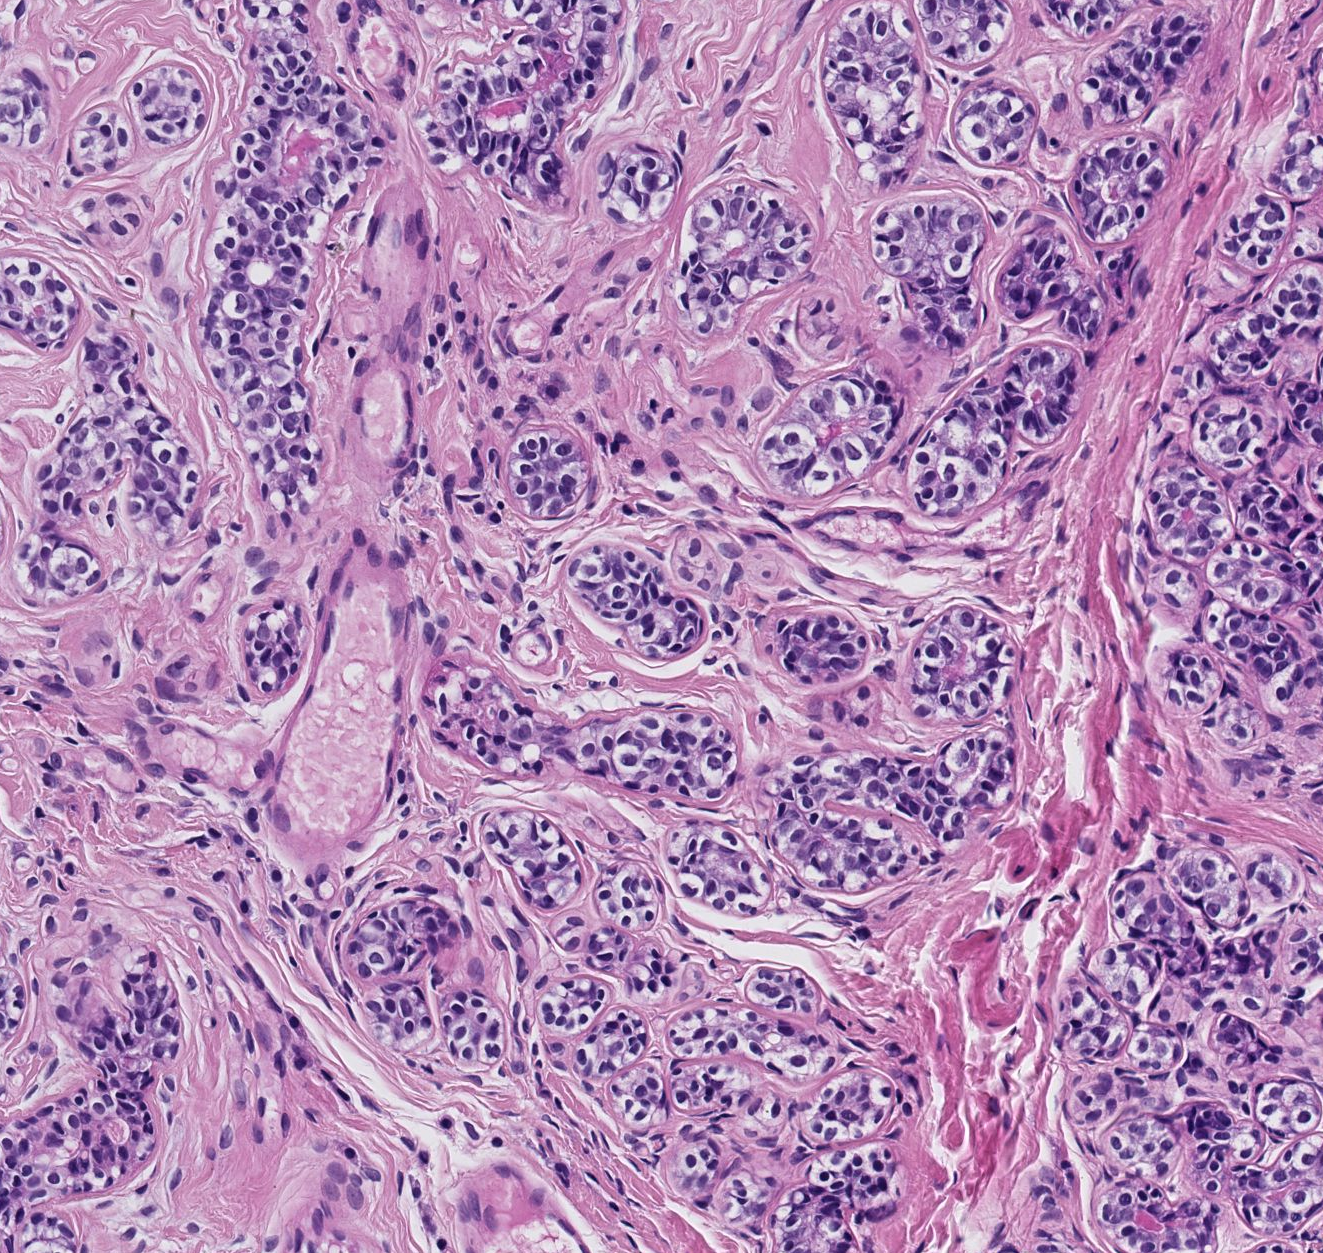
\includegraphics[width=\linewidth]{assets/images/for_presentation/image_100B_[10779, 11621, 12102, 12874].png}
    \caption{TIGER image – JB}
    \label{fig:tiger-jb}
  \end{subfigure}\quad
  \begin{subfigure}[b]{0.32\textwidth}
    \centering
    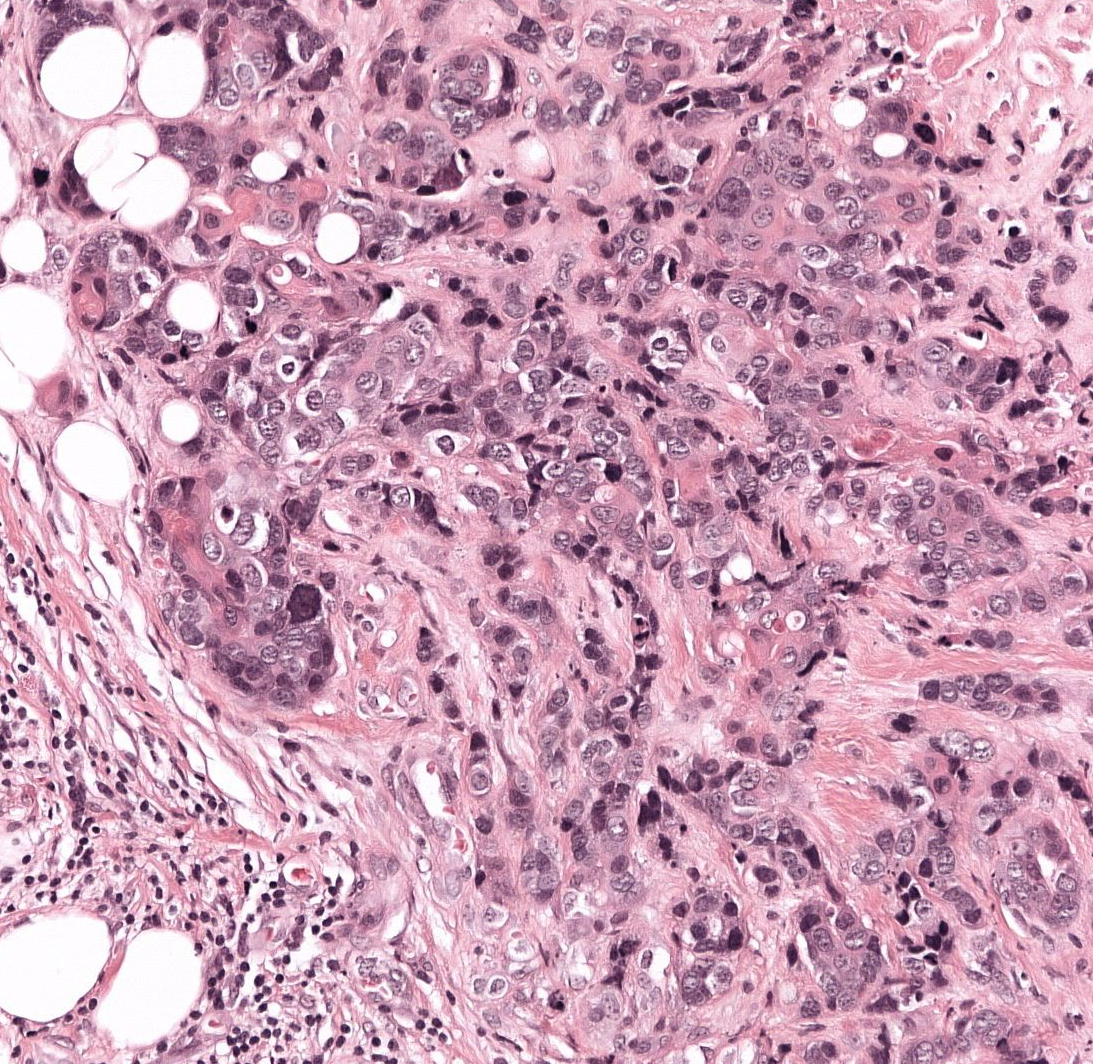
\includegraphics[width=\linewidth]{assets/images/for_presentation/image_TC_S01_P000003_C0001_B104_[50106, 52730, 51199, 53794].png}
    \caption{TIGER image – TC}
    \label{fig:tiger-tc}
  \end{subfigure}

  \par\vspace{1em} % line break with a little vertical space

  % Second row (2 images)
  \begin{subfigure}[b]{0.32\textwidth}
    \centering
    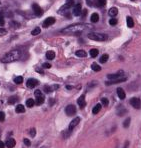
\includegraphics[width=\linewidth]{assets/images/for_presentation/image_TCGA-EW-A1P8-01Z-00-DX1.E9852193-8CDD-49EF-B49B-DA6931198F0D_[8391, 13690, 8532, 13838].png}
    \caption{TIGER image – TCGA}
    \label{fig:tiger-tcga}
  \end{subfigure}\quad
  \begin{subfigure}[b]{0.32\textwidth}
    \centering
    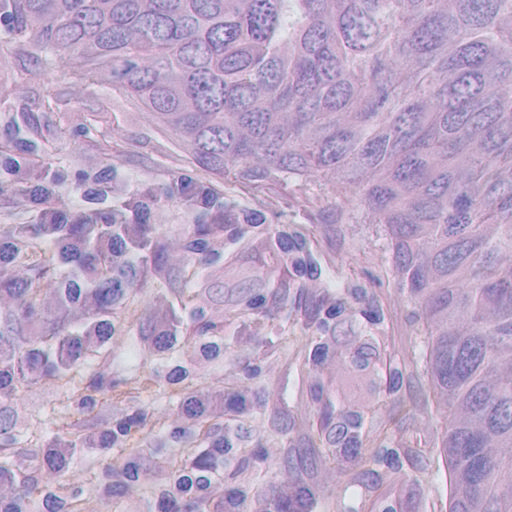
\includegraphics[width=\linewidth]{assets/images/for_presentation/image_10_1.png}
    \caption{TNBC image}
    \label{fig:tnbc}
  \end{subfigure}

  \caption{Example images from TIGER datasets \cite{tiger_dataset} and TNBC \cite{TNBC-nuclei-seg-extended} before normalization.}
  \label{fig:mix-no-norm}
\end{figure}

We employ the multi-target Macenko stain normalization technique as described in \cite{Ivanov2024}, where we select 8 reference images from the TIGER and 2 reference images from the TNBC dataset. This number is arbitrary, but in \cite{Ivanov2024} authors experimented with a different number of reference images (2-20) and showed that the higher number has slightly better results, but if the number is too high, there are no significant improvements. Given the sizes of our respective datasets, we decided to go with the 8 and 2 images. Then we used the same 10 reference images to normalize both datasets. The normalization technique improved the color inconsistencies, as we can see in Figure \ref{fig:mix-norm}.

\begin{figure}[H]
  \centering
  % First row (2 images)
  \begin{subfigure}[b]{0.32\textwidth}
    \centering
    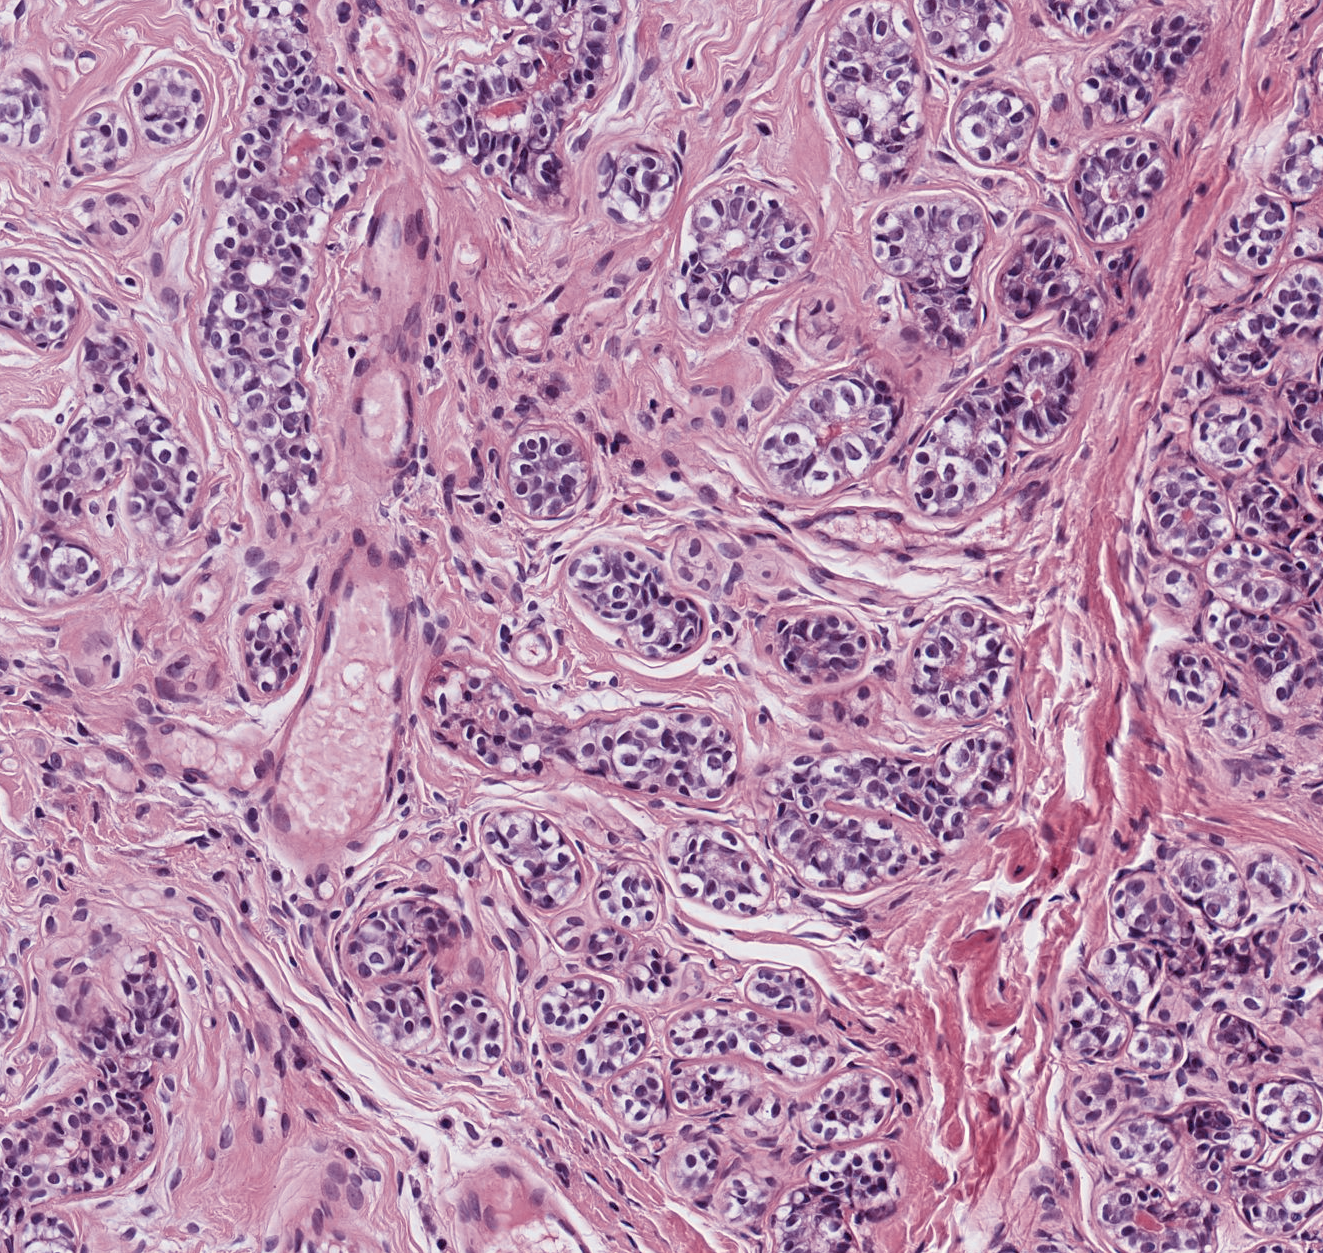
\includegraphics[width=\linewidth]{assets/images/for_presentation/norm_100B_[10779, 11621, 12102, 12874].png}
    \caption{TIGER image – JB}
    \label{fig:tiger-jb}
  \end{subfigure}\quad
  \begin{subfigure}[b]{0.32\textwidth}
    \centering
    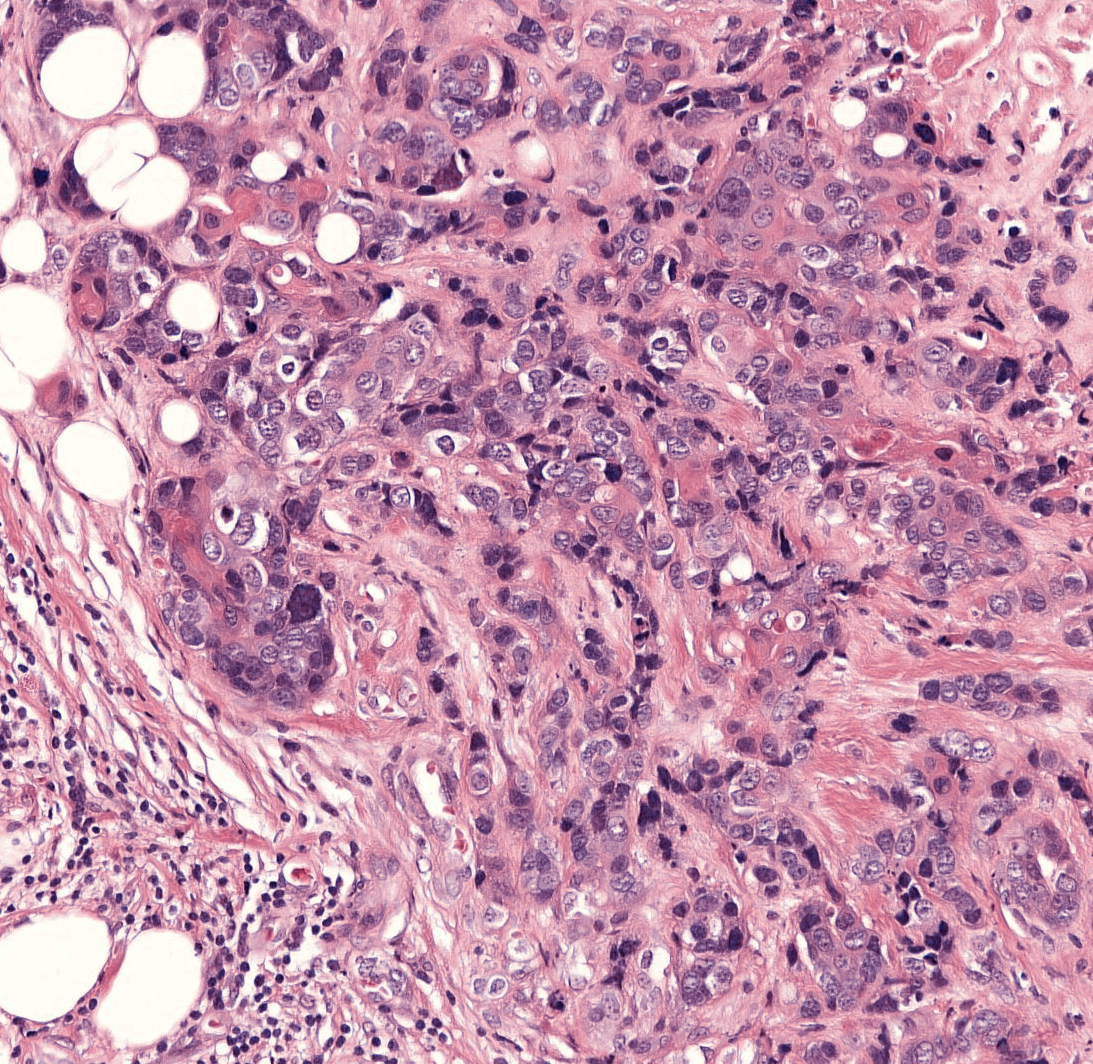
\includegraphics[width=\linewidth]{assets/images/for_presentation/norm_TC_S01_P000003_C0001_B104_[50106, 52730, 51199, 53794].png}
    \caption{TIGER image – TC}
    \label{fig:tiger-tc}
  \end{subfigure}

  \par\vspace{1em} % line break with a little vertical space

  % Second row (2 images)
  \begin{subfigure}[b]{0.32\textwidth}
    \centering
    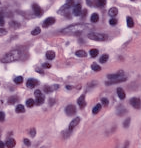
\includegraphics[width=\linewidth]{assets/images/for_presentation/norm_TCGA-EW-A1P8-01Z-00-DX1.E9852193-8CDD-49EF-B49B-DA6931198F0D_[8391, 13690, 8532, 13838].png}
    \caption{TIGER image – TCGA}
    \label{fig:tiger-tcga}
  \end{subfigure}\quad
  \begin{subfigure}[b]{0.32\textwidth}
    \centering
    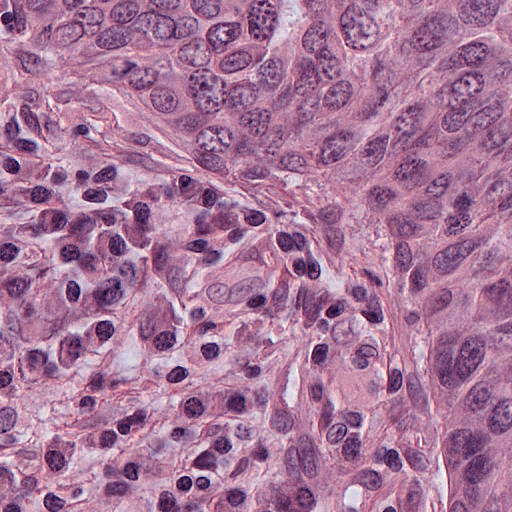
\includegraphics[width=\linewidth]{assets/images/for_presentation/norm_10_1.png}
    \caption{TNBC image}
    \label{fig:tnbc}
  \end{subfigure}

  \caption{Example images from TIGER datasets \cite{tiger_dataset} and TNBC \cite{TNBC-nuclei-seg-extended} after normalization.}
  \label{fig:mix-norm}
\end{figure}

% Image

\subsection{Pseudo-mask sources} 
The next step was to generate the pseudo-masks. For this, we created different variations of the same image. We named the images that were created as a part of one variation \textit{image source}. In total, six different image sources were created for the experiments. We used the original (raw) image as one source, then the normalized image as another source. Furthermore, we extracted the hematoxylin image out of the original image (Macenko normalization does this internally). This was done based on the fact that hematoxylin highlights the cell nuclei, as we described in Chapter \ref{chapter:intro}. This hematoxylin image became our third image source. Lastly, by applying histogram equalization to all of the aforementioned image sources (to increase the overall contrast of the image and shift dark colors into darker ones and light into lighter ones), we obtained another three image sources. The difference in the image sources can be seen in Figure \ref{fig:tiger-sources}. 

\begin{figure}[H]
  \centering
  % First row of three subfigures
  \begin{subfigure}[b]{0.32\textwidth}
    \centering
    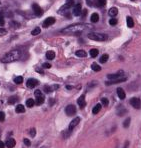
\includegraphics[width=\linewidth]{assets/images/for_presentation/image_TCGA-EW-A1P8-01Z-00-DX1.E9852193-8CDD-49EF-B49B-DA6931198F0D_[8391, 13690, 8532, 13838].png}
    \caption{Original image}\label{fig:tiger-raw}
  \end{subfigure}\hfill
  \begin{subfigure}[b]{0.32\textwidth}
    \centering
    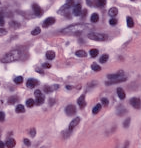
\includegraphics[width=\linewidth]{assets/images/for_presentation/norm_TCGA-EW-A1P8-01Z-00-DX1.E9852193-8CDD-49EF-B49B-DA6931198F0D_[8391, 13690, 8532, 13838].png}
    \caption{Normalized image}\label{fig:tiger-norm}
  \end{subfigure}\hfill
  \begin{subfigure}[b]{0.32\textwidth}
    \centering
    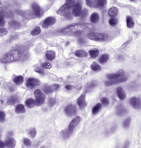
\includegraphics[width=\linewidth]{assets/images/for_presentation/hem_TCGA-EW-A1P8-01Z-00-DX1.E9852193-8CDD-49EF-B49B-DA6931198F0D_[8391, 13690, 8532, 13838].png}
    \caption{Hematoxylin image}\label{fig:tiger-hem}
  \end{subfigure}

  % Line break to start the second row; adjust vertical space as needed
  \par\vspace{1em}

  % Second row of three subfigures
  \begin{subfigure}[b]{0.32\textwidth}
    \centering
    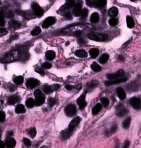
\includegraphics[width=\linewidth]{assets/images/for_presentation/eq_TCGA-EW-A1P8-01Z-00-DX1.E9852193-8CDD-49EF-B49B-DA6931198F0D_[8391, 13690, 8532, 13838].png}
    \caption{Original image with histogram equalization}\label{fig:tiger-eq}
  \end{subfigure}\hfill
  \begin{subfigure}[b]{0.32\textwidth}
    \centering
    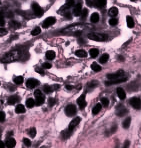
\includegraphics[width=\linewidth]{assets/images/for_presentation/norm_eq_TCGA-EW-A1P8-01Z-00-DX1.E9852193-8CDD-49EF-B49B-DA6931198F0D_[8391, 13690, 8532, 13838].png}
    \caption{Normalized image with histogram equalization}\label{fig:tiger-norm-eq}
  \end{subfigure}\hfill
  \begin{subfigure}[b]{0.32\textwidth}
    \centering
    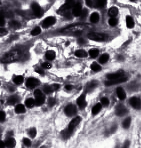
\includegraphics[width=\linewidth]{assets/images/for_presentation/hem_eq_TCGA-EW-A1P8-01Z-00-DX1.E9852193-8CDD-49EF-B49B-DA6931198F0D_[8391, 13690, 8532, 13838].png}
    \caption{Hematoxylin image with histogram equalization}\label{fig:tiger-hem-eq}
  \end{subfigure}
  \caption{Examples of image sources}
  \label{fig:tiger-sources}
\end{figure}


We then operated on each image source with different computer vision techniques to generate the final pseudo-mask PNGs. We describe each of these techniques in the section \ref{section:experiments}. 

\subsection{Aligning the TNBC dataset} 
In order to use the \\ 
TNBC dataset, we needed to align its scale and also the ground truth masks. This dataset was scanned with the $40\times$ magnification; however, the TIGER dataset was scanned using the $20\times$ magnification. To align them, we down-scaled the TNBC dataset images and masks by the factor of 2. Moreover, the 
\\ TNBC ground truth masks were relabeled to binary masks by setting all of the other labels except for the lymphocyte cell labels as background.

\subsection{Patching Strategy}
To be able to feed our data to the deep learning UNet model, we created patches of fixed size $128\times128$ pixels. The TIGER dataset contained images of varying sizes. Therefore, we created overlapping patches with dynamic stride in such a way, that no patch was shifted outside of the original image. We created 19,386 patches of TIGER dataset images. The TNBC dataset was nicer since the original images were of $512\times512$ pixels in size, and after down-scaling by a factor of 2, they became $256\times256$ pixels. Each image was then split into 4 non-overlapping patches. This got us exactly 200 patches of TNBC dataset images. After this stage, the data is ready for the training and evaluation process.

\subsection{Images to Tensors}
For the PyTorch framework to work with the PNG image patches, both original images and masks, we needed to convert them from NumPy arrays into tensors. This was done before the training and evaluation of each trained model.

\section{Evaluation Methods}

\section{Experiments}
\label{section:experiments}
Our proposed system evolved with each performed experiment, since each experiment built on the previous one. We will describe here the architectural setting of each experiment as they followed in order. 

For the first experiment, we utilized just the UNet model itself as a deep learning module, with the preprocessed images from the preprocessing module, as shown in Figure \ref{}. The fully annotated TNBC dataset was used for this task.

The second and third experiments, in addition to the two mentioned above, used the pseudo-label generating module, which was responsible for generating pixel-level masks for each image. The pseudo-labels were generated for the weakly annotated TIGER dataset from the provided bounding box annotations. Those were then used as ground truth masks for subsequent training of the UNet model. The diagram of this architecture is displayed in Figure \ref{}.

The fourth experiment utilized a transfer learning strategy, where we took the model trained during the third experiment and fine-tuned it using part of the fully annotated dataset. This process is visualized in Figure \ref{}.

\subsection{Experiment 1 - Training on Small Dataset with Full Annotations}
setup, diagram, training workflow, results

\subsection{Experiment 2 - Pseudo-mask Generating Strategies}

\subsection{Experiment 3 - Pseudo-mask Fusing Strategies}

\subsection{Experiment 4 - Transfer Learning}

\subsection{Experiments Summary}

\section{Tools}
Python, 
NumPy, 
PyTorch, 
PyTorch Lightning,
Segmentation Models PyTorch, 
Torchstain multitarget macenko norm
Azure ml studio
Jupyter Notebooks
OpenCV
scikit-learn
Weights and Biases
matplotlib.pyplot
PyCharm
Git
GitHub
CUDA